% MAE 263F proposal -- Yuyang Liu.
% Keep this file beside the supplied ieeeconf.cls.
% Embedded bibliography: no .bib file or BibTeX step is required.
% All parameters and performance thresholds are proposed design choices.
\documentclass[letterpaper,10pt,conference]{ieeeconf}
\IEEEoverridecommandlockouts
\overrideIEEEmargins
\usepackage[T1]{fontenc}
\usepackage{amsmath,amssymb,booktabs}
\usepackage{tikz}
\usepackage{algorithm}
\usepackage{algpseudocode}
\usepackage[hidelinks]{hyperref}
\usetikzlibrary{arrows.meta,decorations.pathreplacing}
\newcommand{\vct}[1]{\boldsymbol{#1}}
\newcommand{\pos}[1]{\left\langle #1\right\rangle_{+}}
\title{\LARGE\bf Tendon-Driven Soft Arm:\\Static Positioning and Payload Compensation}
\author{Yuyang Liu\\MAE 263F: Mechanics of Flexible Structures \& Soft Robots\\
University of California, Los Angeles}
\begin{document}
\maketitle
\thispagestyle{empty}
\pagestyle{empty}

\begin{abstract}
A flexible inspection arm can bend to aim a camera or sensor, but the
same tendon command may produce a different tip position after a payload
is attached. This project will develop a planar, two-section
tendon-driven arm simulator for static positioning under gravity.
A discrete elastic beam will represent the backbone, while four
tension-only tendons follow offset guides and anchor at the section
junction or tip. The model will include stretching, bending, tendon
elasticity, self-weight, and a tip payload. Implicit Euler steps with
Newton iteration will relax the arm to equilibrium. A bounded inverse
search will compare replayed unloaded commands with commands recomputed
for the loaded arm. Analytical benchmarks, derivative checks, force
balance, and mesh refinement will verify the implementation. The intended
outcome is a reproducible comparison of positioning accuracy within a
verified feasible workspace.
\end{abstract}

\section{Application and Objectives}
Flexible inspection tools must orient a camera or sensor without bulky
rigid joints. Continuum robots offer distributed bending and structural
compliance, as discussed in soft-robotics and continuum-robot surveys
\cite{rus,burgner}. This project isolates one practical issue: attaching
a tool changes gravitational loading, so commands calibrated without
that tool may no longer reach the intended position.

The task is static tip positioning in a vertical plane. The project
will determine (1) how tendon shortening and payload change equilibrium
shape and reachable positions, and (2) whether load-aware commands reduce
error relative to replaying unloaded commands. Comparisons will use
identical targets and actuator limits. The contribution is an implemented
and verified mechanics-based positioning study, rather than a new rod
theory. Obstacle interaction and a complete inspection system are
outside scope.

\section{Related Work}
Webster and Jones review constant-curvature kinematics for single- and
multisection continuum robots \cite{webster}. This provides a useful
geometric description, but the proposed model will determine curvature
through force balance rather than prescribe it. Trivedi et al.\ include
distributed weight and payload in geometrically exact soft-manipulator
models \cite{trivedi}. Rucker and Webster couple tendon routing to
continuum-robot mechanics under external loads \cite{rucker},
motivating explicit guide and anchor forces.

Bergou et al.\ present a discrete geometric treatment of elastic rods
\cite{bergou}. This project will use the planar beam counterpart taught
in class. Renda et al.\ develop a different discrete Cosserat model for
multisection soft arms \cite{renda}, and Gravagne et al.\ study
large-deflection planar continuum-robot dynamics and control
\cite{gravagne}. These studies provide context; their full
three-dimensional formulations and dynamic controllers will not be
reproduced. The proposed scope retains tendon-induced section coupling
and external loading while restricting the task to planar statics.

\section{Physical System}
\subsection{Geometry and Degrees of Freedom}
The initially straight arm points upward and has two equal sections,
$L_1=L_2=L/2$. Centerline nodes $\vct{x}_i=(x_i,y_i)$ form the
position vector $\vct{q}$. With $N$ active edges and one extra edge
inside the clamp, the system has $N+2$ nodes. Prescribing the first
two nodes at $(0,-h)$ and $(0,0)$, where $h=L/N$, fixes root position and direction,
leaving $2N$ free positional degrees of freedom. Free length $L$
excludes the clamped edge. The section junction is part of a continuous
backbone, not a hinge.

Each section has an opposing tendon pair. The proximal pair anchors
at the junction; the distal pair passes through the proximal section
and anchors at the tip (Fig.~\ref{fig:model}). Distal actuation therefore
also loads the proximal section. Tendons slide through massless,
frictionless guides at offset magnitude $d$. Guide positions and
orientations follow the backbone, adding no independent degrees of
freedom. Cross-section normals use normalized averages of adjacent
edge tangents, with a one-sided tangent at the tip and a prescribed
normal at the fixed root guide. The pairs represent independent tendon
channels even where their planar projections coincide. Dense guiding
is idealized: refining route samples approximates the same continuous
offset path rather than changing the hardware.

\begin{figure}[t]
\centering
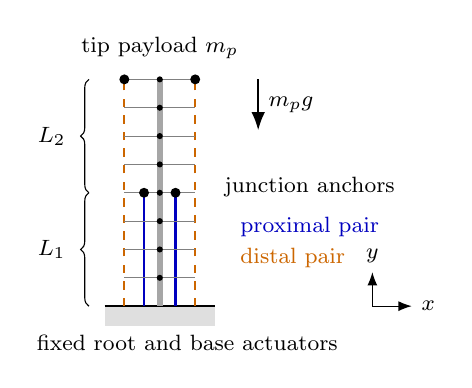
\begin{tikzpicture}[x=1cm,y=0.72cm,>=Latex,font=\footnotesize]
\fill[gray!25] (-0.7,-0.35) rectangle (0.7,0);
\draw[thick] (-0.7,0)--(0.7,0);
\draw[line width=2pt,gray!70] (0,0)--(0,4);
\draw[blue!75!black,thick] (-0.2,0)--(-0.2,2);
\draw[blue!75!black,thick] (0.2,0)--(0.2,2);
\draw[orange!80!black,thick,dashed] (-0.45,0)--(-0.45,4);
\draw[orange!80!black,thick,dashed] (0.45,0)--(0.45,4);
\foreach \y in {0.5,1,1.5,2,2.5,3,3.5,4}{
  \draw[gray] (-0.45,\y)--(0.45,\y);
  \fill (0,\y) circle (1.1pt);
}
\foreach \x/\y in {-0.2/2,0.2/2,-0.45/4,0.45/4}
  \fill (\x,\y) circle (1.8pt);
\draw[decorate,decoration={brace,amplitude=3pt}] (-0.9,0)--(-0.9,2)
  node[midway,left=5pt] {$L_1$};
\draw[decorate,decoration={brace,amplitude=3pt}] (-0.9,2)--(-0.9,4)
  node[midway,left=5pt] {$L_2$};
\node[above] at (0,4.2) {tip payload $m_p$};
\draw[->,thick] (1.25,4)--(1.25,3.1) node[midway,right] {$m_pg$};
\node[anchor=west] at (0.7,2.1) {junction anchors};
\node[anchor=west,text=blue!75!black] at (0.9,1.4) {proximal pair};
\node[anchor=west,text=orange!80!black] at (0.9,0.85) {distal pair};
\node at (0.35,-0.65) {fixed root and base actuators};
\draw[->] (2.7,0)--(3.2,0) node[right] {$x$};
\draw[->] (2.7,0)--(2.7,0.6) node[above] {$y$};
\end{tikzpicture}
\caption{Initial arm and routing. Tendon channels are separated for
visibility; each has offset magnitude $d$. All tendons are base-driven.
Gravity acts downward.}
\label{fig:model}
\end{figure}

\subsection{Energies and External Loading}
For current edge length $\ell_i$ and rest length $\ell_i^0$,
\begin{equation}
E_{\mathrm{arm}}=
\sum_i\frac{EA}{2\ell_i^0}(\ell_i-\ell_i^0)^2+
\sum_i\frac{EI}{2\bar{\ell}_i}(\kappa_i-\kappa_i^0)^2.
\label{eq:beam}
\end{equation}
Here $E,A,I$ are modulus, area, and second moment of area;
$\bar{\ell}_i$ is the mean adjacent rest length. The discrete integrated
curvature is $\kappa_i=2\tan(\phi_i/2)$ for signed turning angle
$\phi_i$; initially $\kappa_i^0=0$. The backbone is geometrically
nonlinear and materially linear elastic, with no shear or twist.

Tendon $a=(j,\sigma)$ is identified by its anchor section
$j\in\{1,2\}$ and side $\sigma\in\{-1,+1\}$. Its guide positions
and routed length are
\begin{equation}
\vct{p}_{a,k}=\vct{x}_{i_k}+\sigma d\,\vct{n}_{i_k},
\qquad
\ell_a(\vct{q})=\sum_k\|\vct{p}_{a,k+1}-\vct{p}_{a,k}\|.
\label{eq:routing}
\end{equation}
Each route starts at its fixed base guide and ends at its anchor.
The commanded free length is
$\ell_a^u=\ell_a^{\mathrm{init}}-\sigma u_j$,
where $\ell_a^{\mathrm{init}}$ is the initial routed length and $u_j$
is signed differential shortening. For $\pos{z}=\max(z,0)$,
\begin{equation}
E_a=\tfrac12K_a\pos{\ell_a-\ell_a^u}^{\,2},
\qquad T_a=K_a\pos{\ell_a-\ell_a^u},
\label{eq:tendon}
\end{equation}
where $K_a$ is tendon axial stiffness in N/m. A tendon can slacken
but never carries compression. Frictionless sliding gives uniform
tension along each tendon. Differentiating its complete path includes
forces and moments at guides and anchors. On a taut branch,
\begin{equation}
\vct{F}_a=-T_a\nabla\ell_a,\qquad
\nabla^2 E_a=K_a\nabla\ell_a\nabla\ell_a^T+T_a\nabla^2\ell_a .
\end{equation}
Slack tendons contribute zero, and the active set is reevaluated
during iteration.

With upward $y$, total potential is
\begin{equation}
\Pi(\vct{q},\vct{u})=E_{\mathrm{arm}}+\sum_a E_a+
\sum_i m_i g y_i+m_p g y_{\mathrm{tip}}.
\end{equation}
The payload also augments tip mass during relaxation. Tendon friction,
contact, and out-of-plane motion are excluded.

\subsection{Starting Parameters}
Table~\ref{tab:parameters} lists numerical design choices, not measured
hardware properties. Pilot runs will check the operating range before
the comparison protocol is frozen. The circular backbone has
$A=\pi r^2$ and $I=\pi r^4/4$.
\begin{table}[t]
\caption{Proposed Starting Values}
\label{tab:parameters}
\centering
\begin{tabular}{@{}ll@{}}
\toprule
Quantity & Value or range\\
\midrule
Free length; section lengths & $0.20$ m; $0.10$ m each\\
Radius; effective modulus & $6$ mm; $10$ MPa\\
Density; gravity & $1000$ kg/m$^3$; $9.81$ m/s$^2$\\
Tendon offset; stiffness & $8$ mm; $1000$ N/m\\
Commands; payload & $u_j\in[-4,4]$ mm; $m_p=0,2,5$ g\\
Active edges & $40$; refinement at $20,80$\\
Initial relaxation step & $\Delta t=0.01$ s\\
\bottomrule
\end{tabular}
\end{table}

\section{Simulation and Positioning Algorithms}
\subsection{Forward Equilibrium}
The implementation will adapt the course's planar beam derivatives
and free-coordinate assembly. Automatic differentiation will evaluate
routing derivatives on each taut/slack branch, checked independently
against finite differences on small problems.

Damped relaxation solves
$\vct{M}\ddot{\vct{q}}+\vct{C}\dot{\vct{q}}+\nabla\Pi=\vct{0}$
with numerical damping $\vct{C}=\gamma\vct{M}$. Implicit Euler gives
\begin{equation}
\begin{split}
\vct{R}={}&\frac{\vct{M}}{\Delta t^2}
(\vct{q}^{n+1}-\vct{q}^n-\Delta t\,\vct{v}^n)\\
&+\frac{\vct{C}}{\Delta t}(\vct{q}^{n+1}-\vct{q}^n)
+\nabla\Pi(\vct{q}^{n+1},\vct{u}),
\end{split}
\end{equation}
with Newton matrix
$\vct{J}=\vct{M}/\Delta t^2+\vct{C}/\Delta t+\nabla^2\Pi$.
Backtracking will limit invalid geometry and reduce the residual.
Failed steps are retried at smaller $\Delta t$; commands are ramped
from accepted states. Iteration and relaxation-step limits will return
an explicit failure status rather than allow indefinite runs.

\begin{algorithm}[t]
\caption{Forward Simulation to Static Equilibrium}
\begin{algorithmic}[1]
\Require Commands $\vct{u}$, payload $m_p$, initial state
\For{each command and load increment}
  \Repeat
    \State Save state; initialize Newton guess
    \Repeat
      \State Evaluate guide paths and taut/slack tendons
      \State Assemble $\nabla\Pi,\nabla^2\Pi,\vct{R},\vct{J}$
      \State Solve $\vct{J}_{ff}\Delta\vct{q}_f=-\vct{R}_f$
      \State Backtrack and update free coordinates
    \Until{step converges or fails}
    \State On failure, reduce $\Delta t$ and retry
    \State Update velocity from the accepted step
  \Until{static force and motion criteria both hold}
\EndFor
\State Check strain, tensions, geometry, and stability
\State \Return Equilibrium, tip position, and status
\end{algorithmic}
\end{algorithm}

Acceptance requires free static force residual below $10^{-5}F_{\rm ref}$
and maximum nodal change below $10^{-5}L$ for 20 consecutive steps,
with decaying velocity. Define
$F_{\rm ref}=\max(EI/L^2,m_{\rm total}g,10^{-3}\,\mathrm{N})$.
Here $m_{\rm total}$ includes backbone and payload mass. The free
potential Hessian will be checked for stability; switching
states will receive additional perturbation checks. Numerical damping
is solely a route to static equilibrium. Physical settling time and
damping are not evaluation outputs.

\subsection{Inverse Positioning and Comparison}
Let $\vct{p}(\vct{u},m_p)$ be the converged tip position.
Bounded nonlinear least squares will minimize
\begin{equation}
\frac{\|\vct{p}(\vct{u},m_p)-\vct{p}^*\|^2}{L^2}
+\lambda\frac{\|\vct{u}\|^2}{u_{\max}^2},
\qquad |u_j|\leq u_{\max},
\end{equation}
initially using $\lambda=10^{-6}$. Finite differences of converged
forward solves give tip sensitivities. Several starting commands from
a coarse scan will reduce local-minimum sensitivity.

A $9\times9$ command scan and local refinement will identify stable
operating regions. Ten to fifteen non-collinear targets will be chosen
in the common verified workspace of unloaded and loaded arms.
Nearly singular command-to-tip mappings, especially near the straight
pose, will be flagged. Provisional limits of 2 N tendon tension and
2\% backbone axial strain will exclude invalid states, as will
self-intersection or nearly reversed adjacent edges. Limits and target
rules will remain fixed during the comparison.

For each target, unloaded command $\vct{u}_0$ will be replayed on the
loaded arm, then a load-aware command $\vct{u}_{m_p}$ will be computed.
Errors are
\begin{equation}
\begin{split}
e_{\rm replay}&=\|\vct{p}(\vct{u}_0,m_p)-\vct{p}^*\|,\\
e_{\rm comp}&=\|\vct{p}(\vct{u}_{m_p},m_p)-\vct{p}^*\|.
\end{split}
\end{equation}
Outputs will include mean and maximum error, successful-target
fraction, tensions, and solve cost. An error below 1\% of arm length
is a proposed goal, not a claimed result. Commands will also be
evaluated on a finer mesh. Forward failures will be recorded rather
than interpreted as valid positions. The payload is known; the task
is model-based command compensation, not online load estimation.

\section{Validation and Expected Results}
Verification will precede positioning experiments.
\begin{enumerate}
\item \textit{Beam benchmarks:} Disable tendons and gravity. For a
small transverse tip force $F$, compare displacement with
$FL^3/(3EI)$. In a separate small end-moment test, compare rotation
and displacement with $ML/(EI)$ and $ML^2/(2EI)$.
\item \textit{Tendon and derivative checks:} Verify zero compression
force, $T=K_a\Delta\ell$ on a fixed straight route, and virtual work
$\delta E_a=T_a\delta\ell_a$ at fixed command. Check energy gradients
and Hessian-vector products by centered differences away from
taut/slack transitions.
\item \textit{Balance and refinement:} Check root reactions, gravity,
and base-tendon forces, including moment balance. Refine active edges
from 20 to 40 to 80 at fixed physical dimensions. Proposed goals are
less than $0.01L$ tip-position change and 5\% taut-tendon-tension
change between the last two meshes. Repeat representative cases with
halved time steps and different numerical damping.
\end{enumerate}
Expected outputs are shape animations, workspace maps, tendon-tension
curves, and paired error plots. The hypothesis is that payload changes
the command-to-position mapping and that load-aware commands reduce
error for feasible targets. Small improvements and failed cases will
be reported. These tests verify implementation; quantitative prediction
for real hardware would require material calibration and experiments.

\section{Work Plan and Deliverables}
Stage 1 will implement a single section, tendon routing, and analytical
and derivative tests. Stage 2 will add the distal pair, verify coupling,
and complete mesh and workspace studies. Stage 3 will perform inverse
positioning and payload comparisons, followed by the report and
presentation. Single-section operation is an intermediate milestone;
the final goal remains the two-section arm.

Deliverables will include Python forward and positioning solvers,
reproducible validation cases, saved comparison data and figures, and
a README. Adapted course routines will retain attribution. The report
will state assumptions and unsuccessful cases. Hardware fabrication,
friction, contact, three-dimensional motion, and dynamic tracking are
excluded from the required scope.

% The separate bibliography does not count toward the body-page limit.
% IEEE numbered references are consistent with the supplied template.
\clearpage
\begin{thebibliography}{8}
\bibitem{rus}
D. Rus and M. T. Tolley, ``Design, fabrication and control of soft robots,''
\emph{Nature}, vol. 521, no. 7553, pp. 467--475, 2015,
doi: \href{https://doi.org/10.1038/nature14543}{10.1038/nature14543}.
\bibitem{burgner}
J. Burgner-Kahrs, D. C. Rucker, and H. Choset,
``Continuum robots for medical applications: A survey,''
\emph{IEEE Transactions on Robotics}, vol. 31, no. 6,
pp. 1261--1280, 2015,
doi: \href{https://doi.org/10.1109/TRO.2015.2489500}{10.1109/TRO.2015.2489500}.
\bibitem{webster}
R. J. Webster III and B. A. Jones,
``Design and kinematic modeling of constant curvature continuum robots:
A review,'' \emph{The International Journal of Robotics Research},
vol. 29, no. 13, pp. 1661--1683, 2010,
doi: \href{https://doi.org/10.1177/0278364910368147}{10.1177/0278364910368147}.
\bibitem{trivedi}
D. Trivedi, A. Lotfi, and C. D. Rahn,
``Geometrically exact models for soft robotic manipulators,''
\emph{IEEE Transactions on Robotics}, vol. 24, no. 4,
pp. 773--780, 2008,
doi: \href{https://doi.org/10.1109/TRO.2008.924923}{10.1109/TRO.2008.924923}.
\bibitem{rucker}
D. C. Rucker and R. J. Webster III,
``Statics and dynamics of continuum robots with general tendon routing
and external loading,'' \emph{IEEE Transactions on Robotics},
vol. 27, no. 6, pp. 1033--1044, 2011,
doi: \href{https://doi.org/10.1109/TRO.2011.2160469}{10.1109/TRO.2011.2160469}.
\bibitem{bergou}
M. Bergou, M. Wardetzky, S. Robinson, B. Audoly, and E. Grinspun,
``Discrete elastic rods,'' in \emph{ACM SIGGRAPH 2008 Papers},
2008, pp. 1--12,
doi: \href{https://doi.org/10.1145/1399504.1360662}{10.1145/1399504.1360662}.
\bibitem{renda}
F. Renda, F. Boyer, J. Dias, and L. Seneviratne,
``Discrete Cosserat approach for multisection soft manipulator dynamics,''
\emph{IEEE Transactions on Robotics}, vol. 34, no. 6,
pp. 1518--1533, 2018,
doi: \href{https://doi.org/10.1109/TRO.2018.2868815}{10.1109/TRO.2018.2868815}.
\bibitem{gravagne}
I. A. Gravagne, C. D. Rahn, and I. D. Walker,
``Large deflection dynamics and control for planar continuum robots,''
\emph{IEEE/ASME Transactions on Mechatronics}, vol. 8, no. 2,
pp. 299--307, 2003,
doi: \href{https://doi.org/10.1109/TMECH.2003.812829}{10.1109/TMECH.2003.812829}.
\end{thebibliography}
\end{document}
